\documentclass[12pt,a4paper]{article}

% 如果需要中文支持,推荐使用xeCJK + 字体设置
\usepackage{xeCJK}
\setCJKmainfont{SimSun}  % 示例:宋体,可根据系统字体情况更换
\usepackage{amsmath}      % 数学公式(如有需要)
\usepackage{graphicx}     % 插图
\usepackage{geometry}     % 调整页边距
\usepackage{fancyhdr}     % 自定义页眉页脚
\usepackage{indentfirst}  % 中文首行缩进
\usepackage{calc}         % 允许做长度运算(测量文字宽度等)
\usepackage{titlesec}
\usepackage{booktabs} % 解决 \midrule 和 \bottomrule 报错
\usepackage{enumitem} % 支持自定义列表格式
\usepackage{float}
\usepackage{subcaption}


% 设置 \section 级标题为:加粗、大字号(如 \Large)
\titleformat{\section}
	{\bfseries\large}    % 标题自身的格式
	{\thesection}        % 标题编号的显示方式
	{1em}                % 编号与标题文字之间的间距
	{}                   % 在标题文字前后可插入额外代码,此处为空
	
% 设置 \subsection 级标题为:加粗、中等字号(如 \normalsize)
\titleformat{\subsection}
	{\bfseries\normalsize}
	{\thesubsection}
	{1em}
{}

% 页面设置(可根据需要微调)
\geometry{
	left=2cm,
	right=2cm,
	top=1cm,
	bottom=1.5cm
}

% 不需要过大的行距,使用较接近单倍行距的设置
\renewcommand{\baselinestretch}{1}

% 仅在页脚居中显示页码,页眉保持为空
\pagestyle{fancy}
\fancyhf{}  % 清空默认的页眉页脚
\fancyfoot[C]{\thepage}
\renewcommand{\headrulewidth}{0pt}
\renewcommand{\footrulewidth}{0pt}

% 首行缩进2字符(中文习惯)
\setlength{\parindent}{0pt}
\setlength{\leftskip}{2em}

\begin{document}
	%-------------------------------------------------------
	% 1 并排两个minipage:左标题、右校徽
	%   - 0.65\textwidth + 0.35\textwidth = \textwidth
	%   - 如果校徽过大或过小,可改宽度,如 0.25\textwidth、0.3\textwidth 等
	%   - 如果想让标题更大,可将 \Huge 改成 \huge 或 \LARGE
	%-------------------------------------------------------
	\noindent
	\hspace{-2em}
	\begin{minipage}[c]{0.65\textwidth}
		\raggedright
		{\fontsize{40pt}{60pt}\selectfont 物理实验报告}
	\end{minipage}
	\begin{minipage}[c]{0.35\textwidth}
		\raggedleft
		% 强制把校徽拉大到 0.35\textwidth 宽度 (高度自动匹配)
		% 若想指定高度,可用 "height=3cm" 等. 二选一即可.
		
\includegraphics[width=\linewidth, trim={20cm 20cm 20cm 20cm}, clip]{university_logo.png}
	\end{minipage}

	\vspace{-1em}
	

	%下方画两条分割线,并在两线之间写学号、姓名、日期、时间
	
	\hrule
	\vspace{0.4em}
	\noindent
	\begin{tabular}{l l l l}
    学号:\underline{114514} & 姓名:\underline{SUSTech} &
    日期:\underline{2025/03/01} & 时间:\underline{周二下午}
	\end{tabular}
	\vspace{-0em}
	\par
	\hrule

	

	%正文示例

	
	\section{实验名称:示波器原理及其应用}
	
	\section{实验目的}
	1. 了解示波器的基本结构和原理\\
	2. 学习使用示波器观察波形和测量信号周期及时间参数等。


	\section{实验原理}
	示波器主要由示波管和相关的电子线路构成,其基本结构如图所示。
		\begin{figure}[htbp]
		\centering
		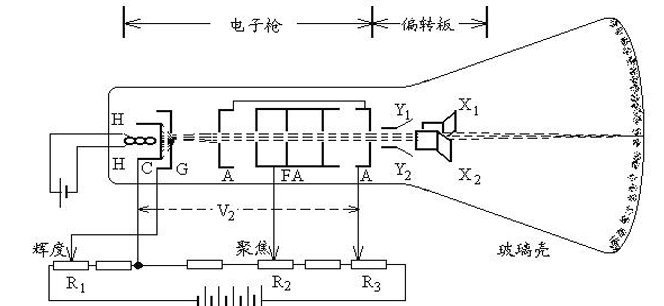
\includegraphics[width=0.3\textwidth]{示波管示意图.png}
		\caption{示波管示意图}
		\label{fig:chart1}
		\end{figure}
	
		\setcounter{section}{3}
		\subsection{偏转电场控制电子束在视屏上的轨迹}
		偏转电压U与偏转位移Y(或X)成正比关系。如果只在竖直偏转板(Y轴)上加一正弦电压,则电子只在竖直方向随电压变化而往复运动。要能够显示波形,必须在水平偏转板(X轴)上加一扫描电压。
			\begin{figure}[htbp]
			\centering
			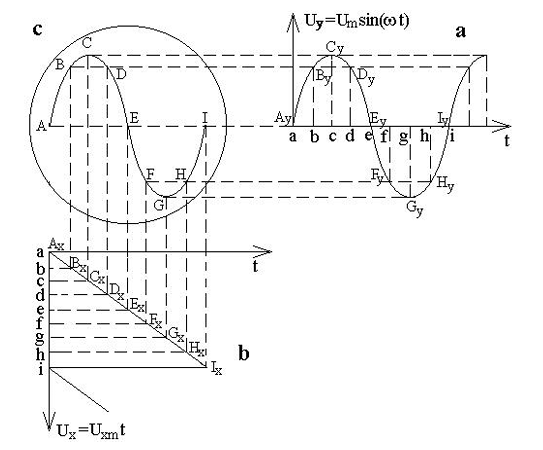
\includegraphics[width=0.40\textwidth]{示波器显示波形原理图.png}
			\caption{示波器显示波形原理图}
			\label{fig:chart1}
			\end{figure}

		\subsection{同步扫描}
		若没有“扫描”,则显示不出信号随时间的变化;若没有“整步”,则得不到稳定的信号图象。示波器常有三种整步形式:
		\begin{enumerate}
			\item “内整步”:将待测信号一部分加到扫描发生器,它使扫描频率 $f_x$ 追随外信号 $f_y$ 的变化而变化;
			\item “外整步”:从外部电路取出信号至扫描发生器追踪;
			\item “电源整步”:从电源变压器取得整步信号。一般观察时采用内整步(又称触发)。
		\end{enumerate}

		\subsection{李萨如图形}
		实质:沿Y轴方向的简谐运动与沿X轴方向的简谐振动合成的一种合运动
		两信号频率相同,振幅(相位)不同时,会产生图2.3所示的(类)椭圆曲线;两信号相位差一定,频率比为有理数时,会产生稳定闭合曲线。该曲线可用于测量两信号的频率比:$\frac{f_x}{f_y} = \frac{n_x}{n_y}$
		其中 $n_x, n_y$ 分别为图形在水平方向和竖直方向上的叶数(即外切线的切点数)。

		\subsection{测正弦波的峰-峰值Vpp、周期T}
		若信号正负峰间为$a$格、周期宽度为$b$格,扫描参数为$v$(V/div) 和 $t$ (s/div),则 $V_{pp} = av, T = bt$。


	
	\section{实验仪器}
		双踪示波器,函数信号发生器,接线板,导线若干

	\section{实验内容}
	\setcounter{section}{5}
	\setcounter{subsection}{0}
	\subsection{用示波器测量信号的周期与幅度}
	\begin{enumerate}
    \item 测量示波器自带校准信号的周期与幅度,并与理论值比较 \\
	0.1ms/div 更好;在能看到完整波形的前提下,时基越小,长度越长,读数误差越小,数据越准确。
    \item 信号发生器产生 $f=2000\,\mathrm{Hz},\, V_{pp}=0.5\,\mathrm{V},\, 1\,\mathrm{V},\, 1.5\,\mathrm{V},\, 2\,\mathrm{V},\, 2.5\,\mathrm{V},\, 3\,\mathrm{V},\, 3.5\,\mathrm{V}$ 的正弦波,分别接示波器 Y 输入口,选择示波器合适的灵敏度,测量信号幅度,并作测得的幅度 $y(V_{pp})$ —— 发生幅度 $x(V_{pp})$ 曲线。
    \item 信号发生器产生 $V_{pp}=5\,\mathrm{V},\, f=0.2,\, 0.5,\, 1.2,\, 5,\, 10,\, 20\,\mathrm{kHz}$ 的正弦波,分别接示波器 Y 输入口,选择示波器合适的时基,测量信号周期,换算为频率,并作测得频率 $y(\mathrm{kHz})$ —— 发生频率 $x(\mathrm{kHz})$ 曲线。
	\end{enumerate}

	\subsection{观察李萨如图形并测频率}
	信号发生器两通道分别产生正弦波接示波器 X、Y,取 $f_x=1200\,\mathrm{Hz}$ 。调节$f_y,\, \phi_y$获得李萨如图形,记录相应的 $f_y,\, \phi_y$ 与图形,验证上述关系式。

	
	\section{数据记录与处理}
	\setcounter{section}{6}
	\setcounter{subsection}{0}
	根据实验结果记录数据,并使用excel整合处理
		\begin{figure}[H]
		\centering
		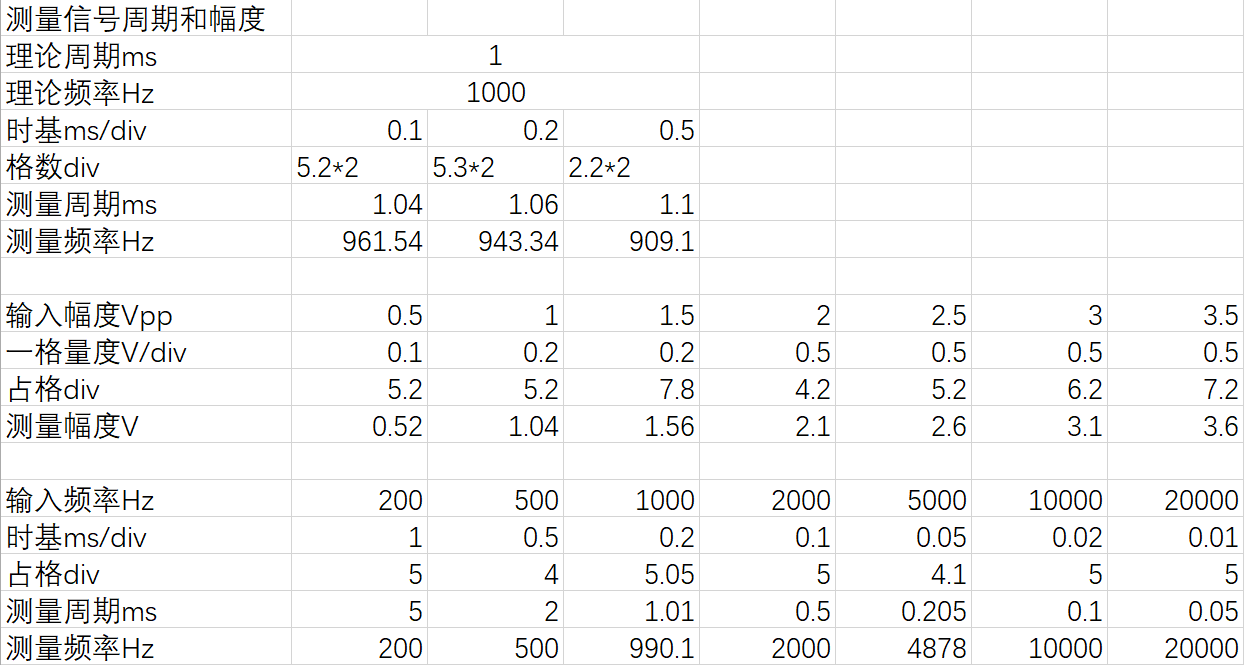
\includegraphics[width=0.40\textwidth]{数据.png}
		\caption{数据记录}
		\label{fig:chart1}
		\end{figure}

	\subsection{用示波器测量信号的周期与幅度}
	根据以上数据,绘制测得幅度-发生幅度曲线及测得频率-发生频率曲线,如下图:
	\begin{figure}[H]
		\centering
		\begin{subfigure}[b]{0.4\textwidth}
			\centering
			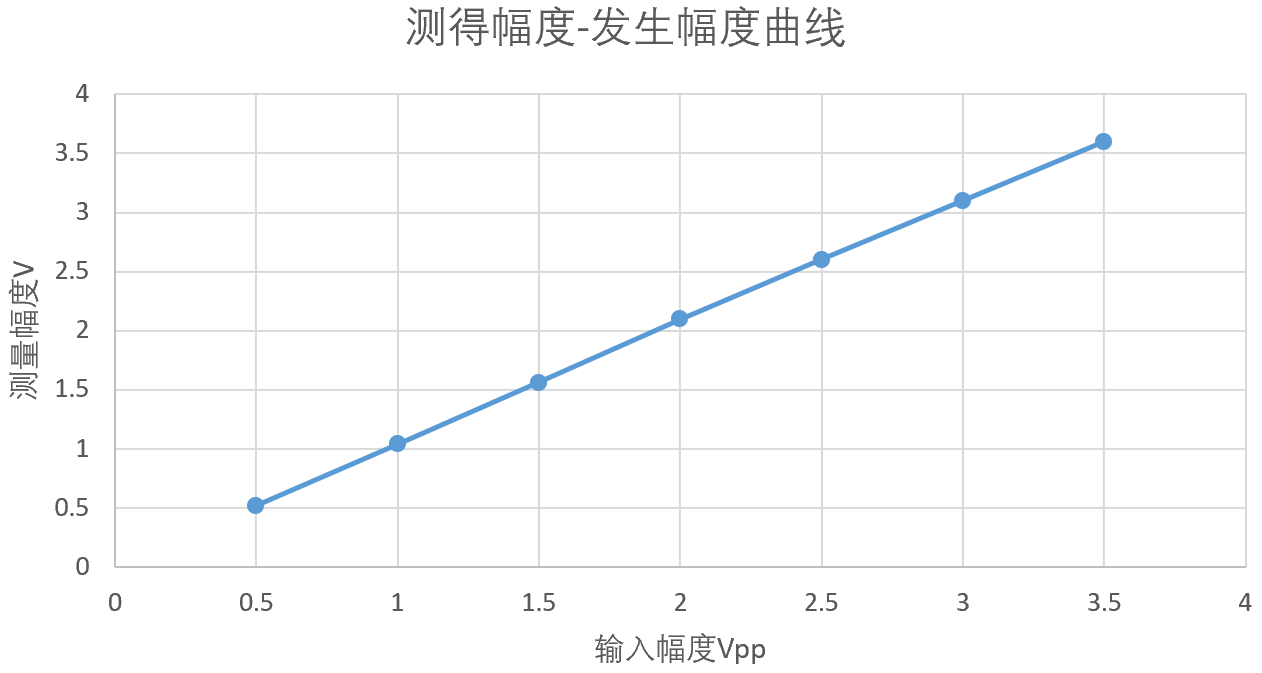
\includegraphics[width=\textwidth]{测得幅度-发生幅度曲线.png}
			\caption{测得幅度-发生幅度曲线}
			\label{fig:chart-amplitude}
		\end{subfigure}
		\hfill
		\begin{subfigure}[b]{0.4\textwidth}
			\centering
			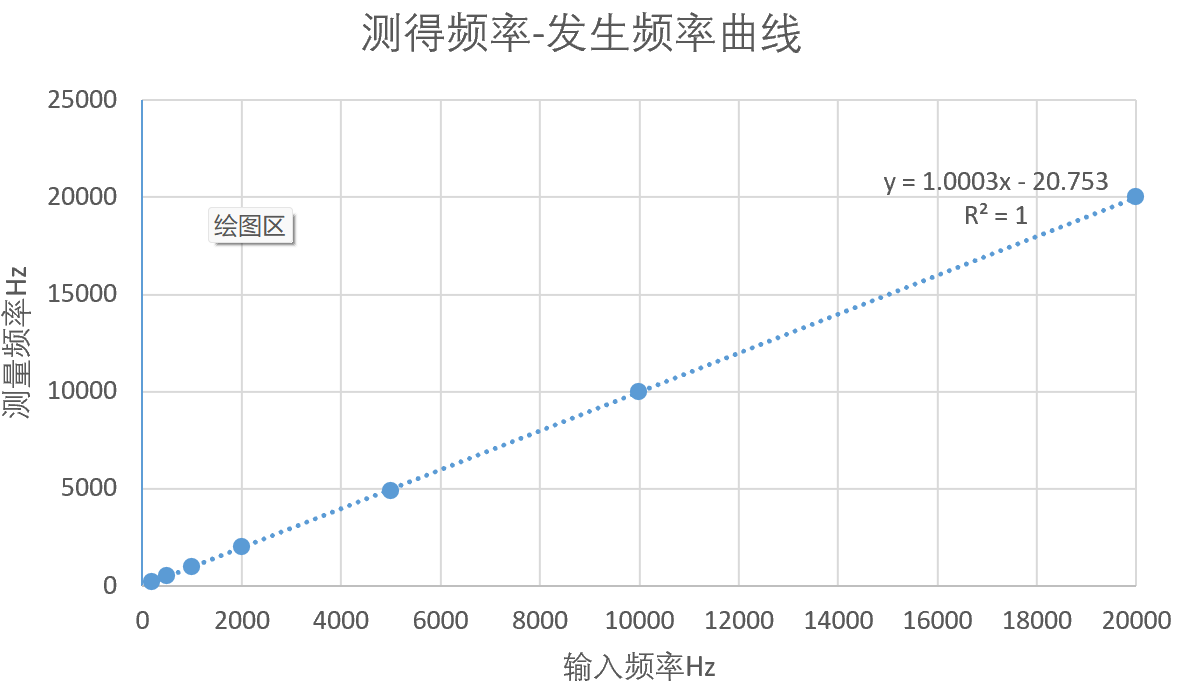
\includegraphics[width=\textwidth]{测得频率-发生频率曲线.png}
			\caption{测得频率-发生频率曲线}
			\label{fig:chart-frequency}
		\end{subfigure}
		\caption{测得幅度与发生幅度、测得频率与发生频率曲线}
		\label{fig:chart1}
	\end{figure}	

	\subsection{观察李萨如图形并测频率}
	同频率不同相位的李萨如图形 \quad $f_x=f_y=1200\,\mathrm{Hz}$
	\begin{figure}[H]
		\centering
		% 第一组:逐步变化的相位差图(以π/4间隔),两行展示,每行4幅图像
		% 第一行
		\begin{subfigure}[b]{0.23\textwidth}
			\centering
			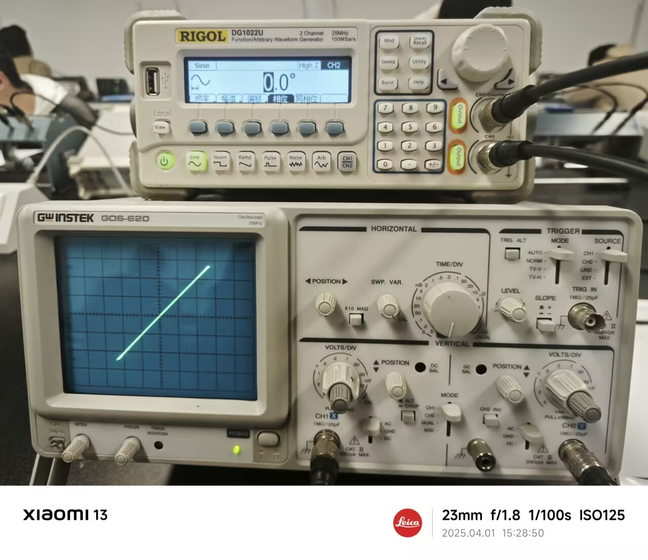
\includegraphics[width=\textwidth]{0.jpg}
			\caption{$\phi_1-\phi_2=0$}
			\label{fig:sub0}
		\end{subfigure}
		\hfill
		\begin{subfigure}[b]{0.23\textwidth}
			\centering
			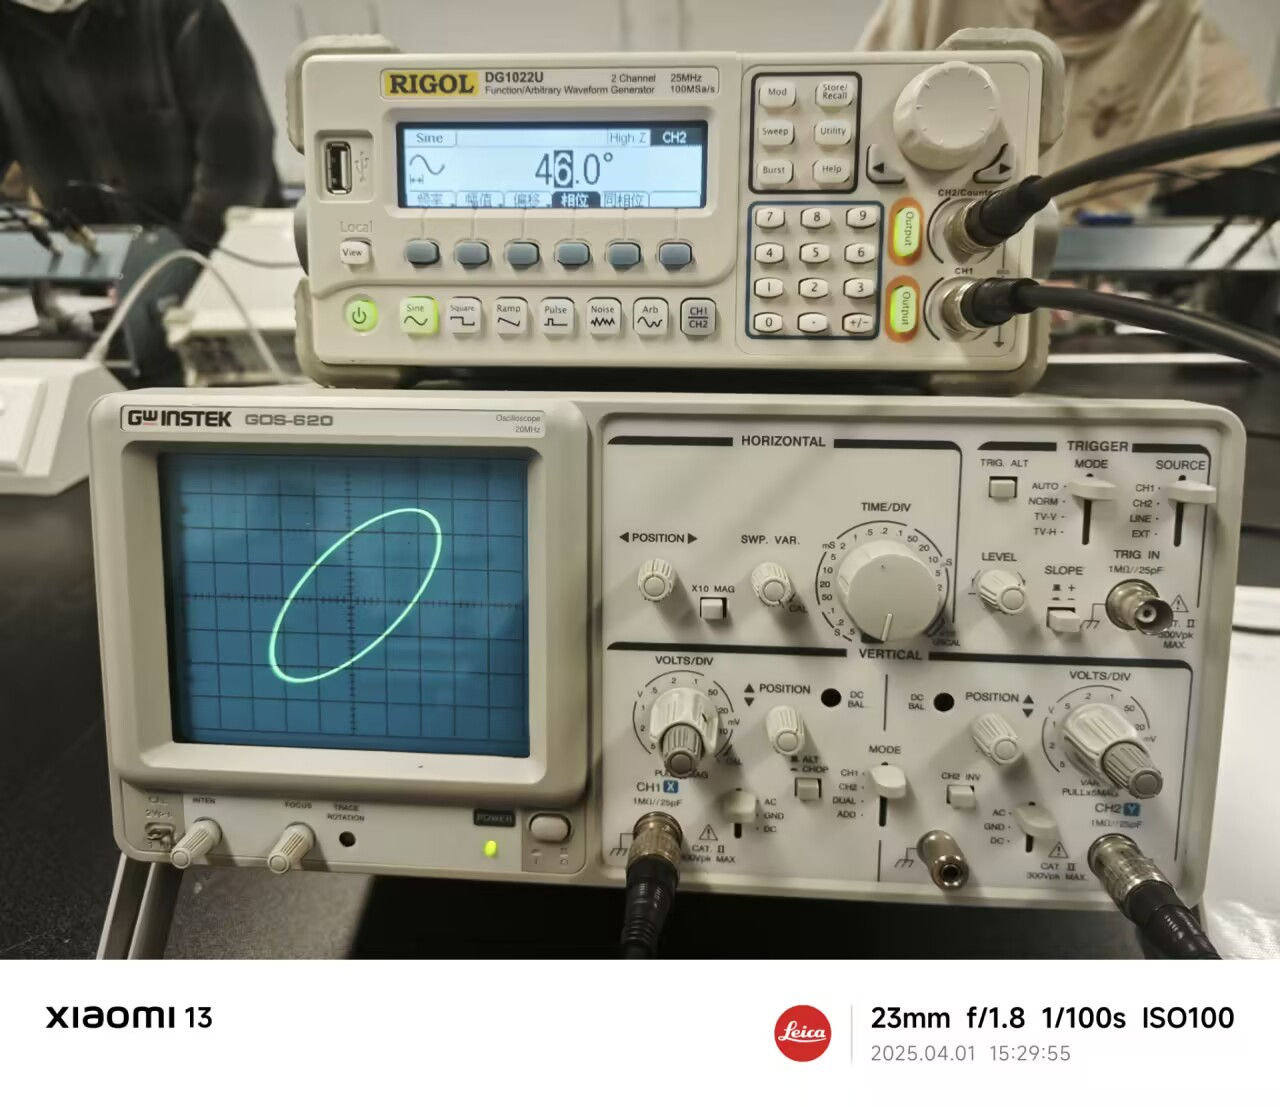
\includegraphics[width=\textwidth]{45.jpg}
			\caption{$\phi_1-\phi_2=\pi/4$}
			\label{fig:subpi4}
		\end{subfigure}
		\hfill
		\begin{subfigure}[b]{0.23\textwidth}
			\centering
			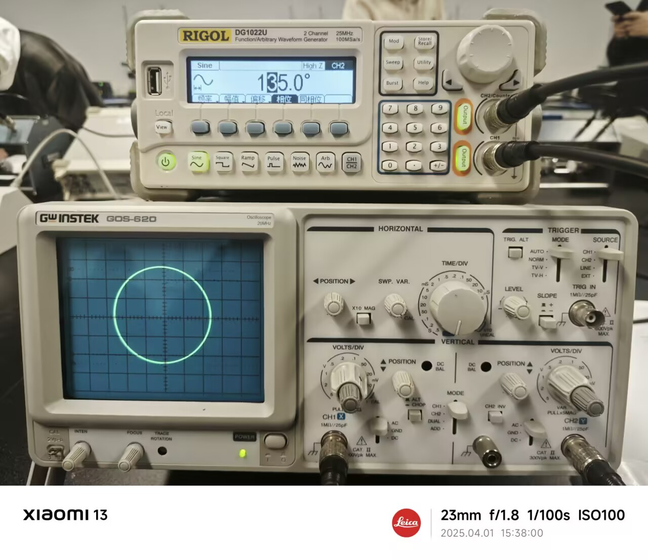
\includegraphics[width=\textwidth]{90.jpg}
			\caption{$\phi_1-\phi_2=\pi/2$}
			\label{fig:subpi2}
		\end{subfigure}
		\hfill
		\begin{subfigure}[b]{0.23\textwidth}
			\centering
			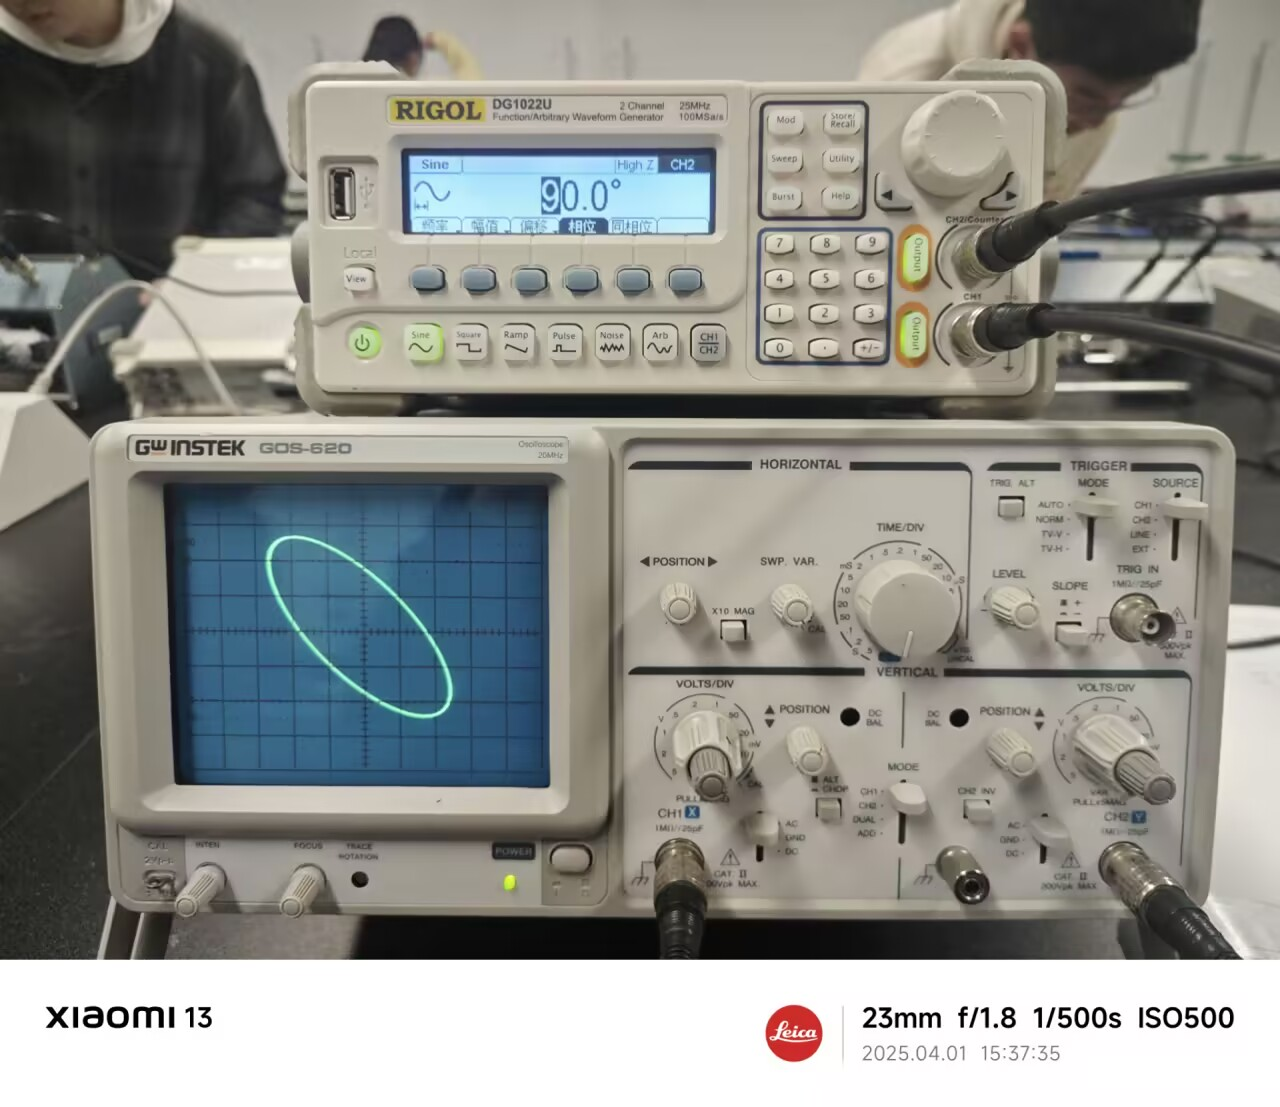
\includegraphics[width=\textwidth]{135.jpg}
			\caption{$\phi_1-\phi_2=3\pi/4$}
			\label{fig:sub3pi4}
		\end{subfigure}
		
		\vspace{1em}
		
		% 第二行
		\begin{subfigure}[b]{0.23\textwidth}
			\centering
			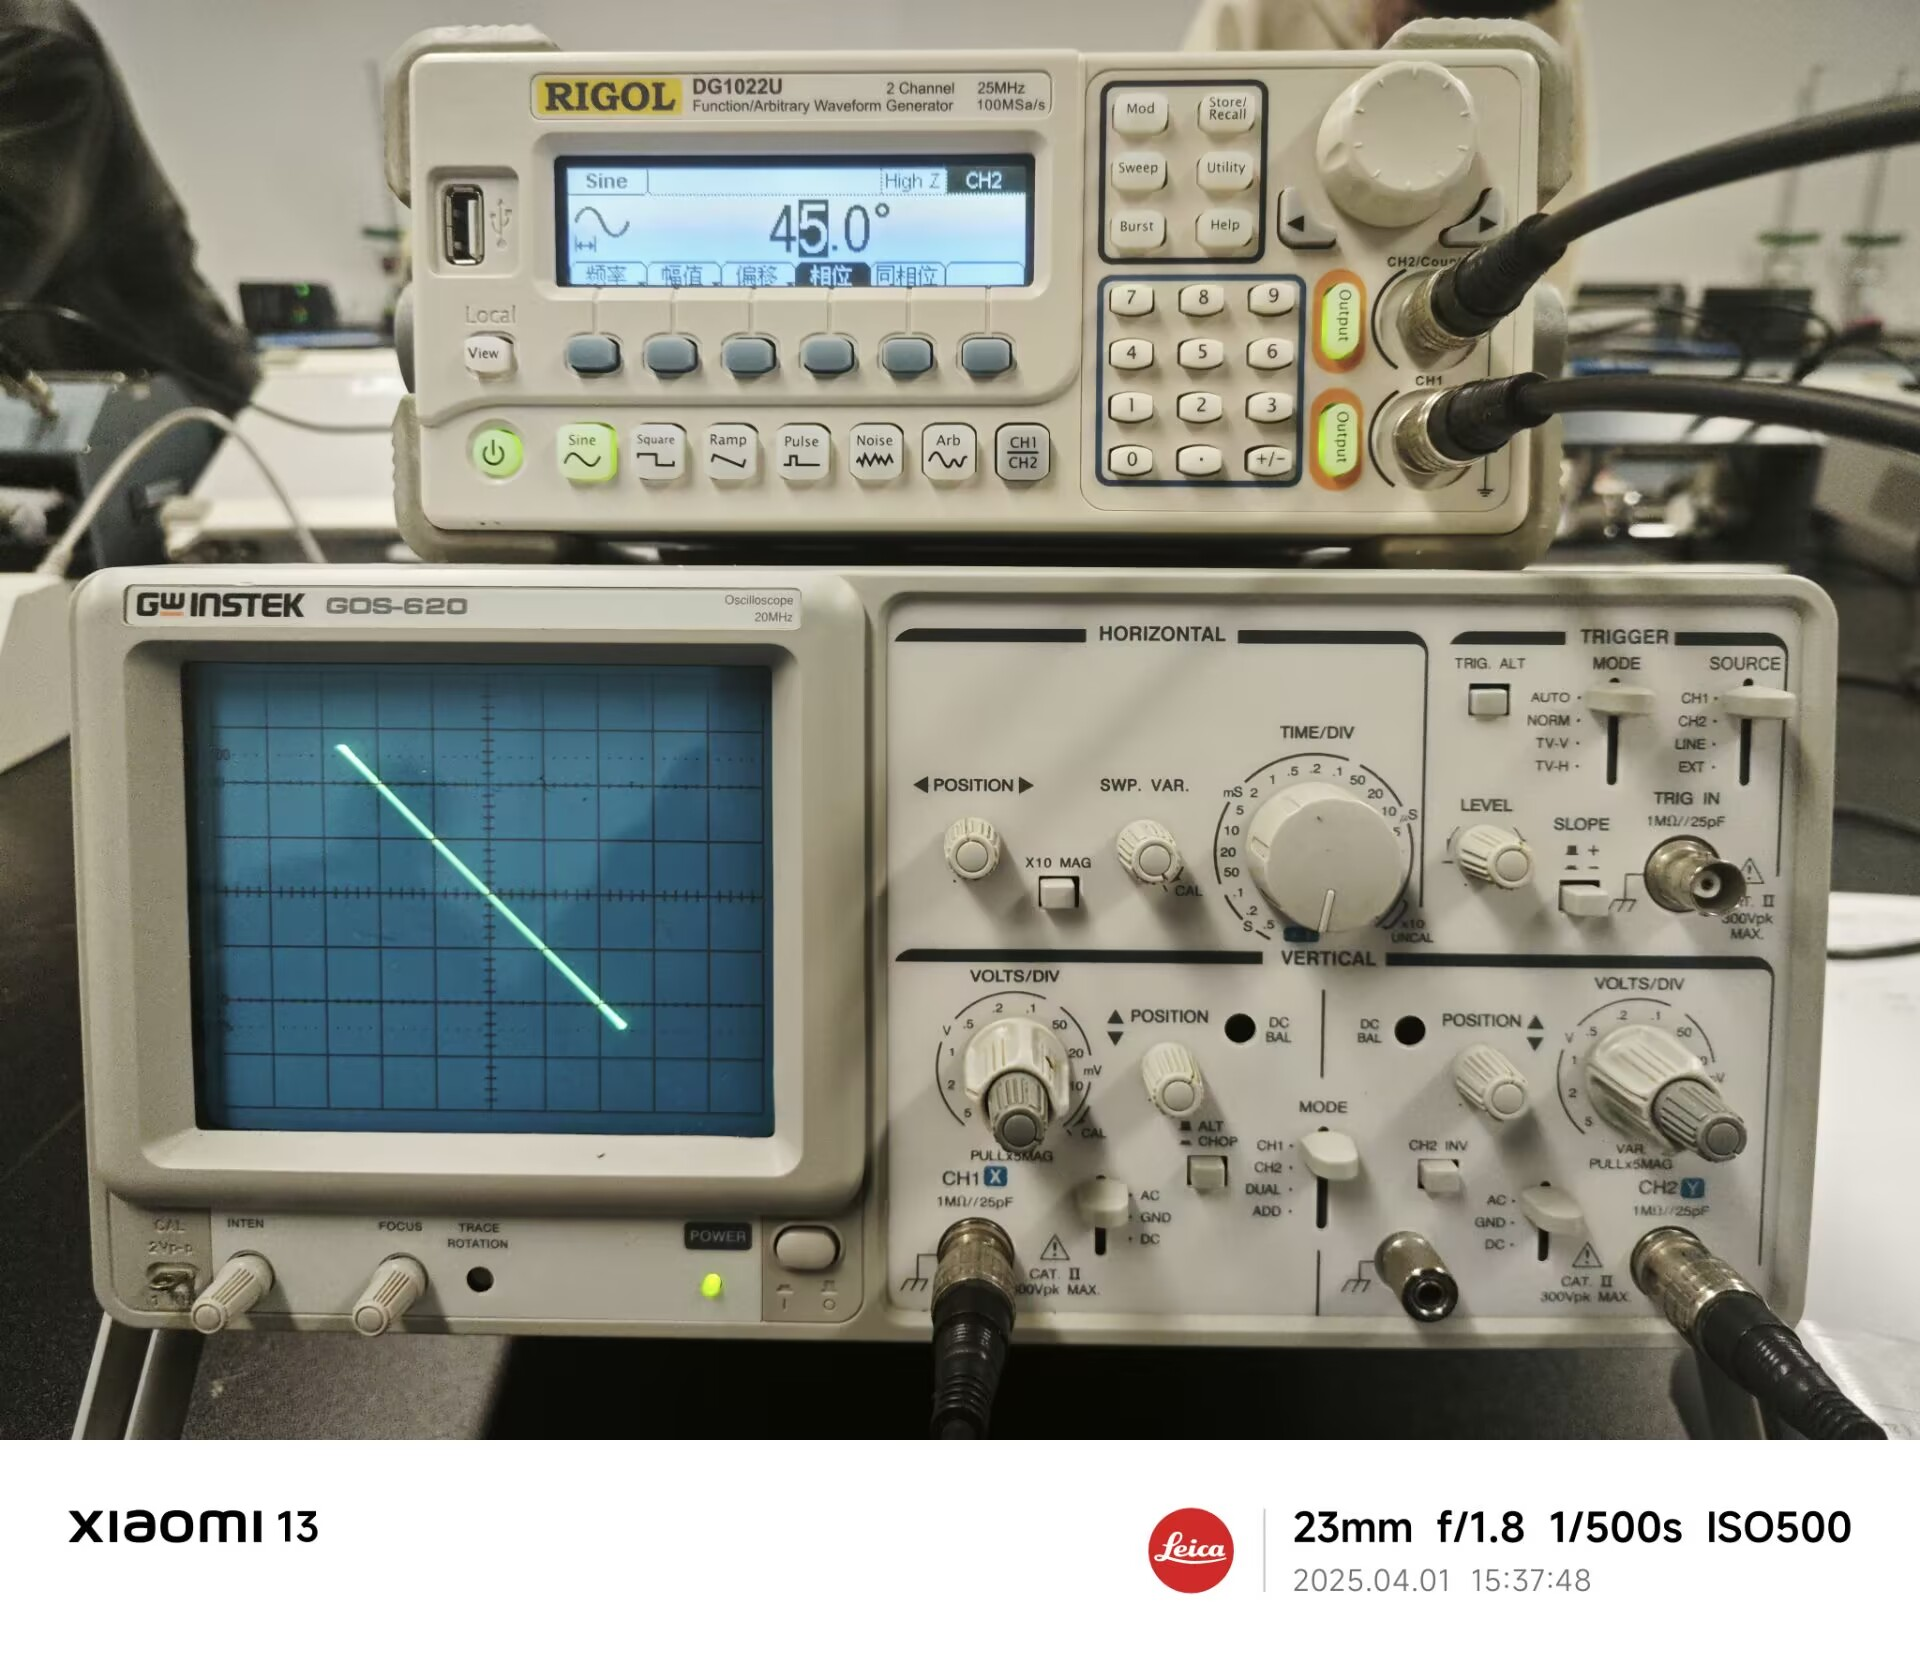
\includegraphics[width=\textwidth]{180.jpg}
			\caption{$\phi_1-\phi_2=\pi$}
			\label{fig:subpi}
		\end{subfigure}
		\hfill
		\begin{subfigure}[b]{0.23\textwidth}
			\centering
			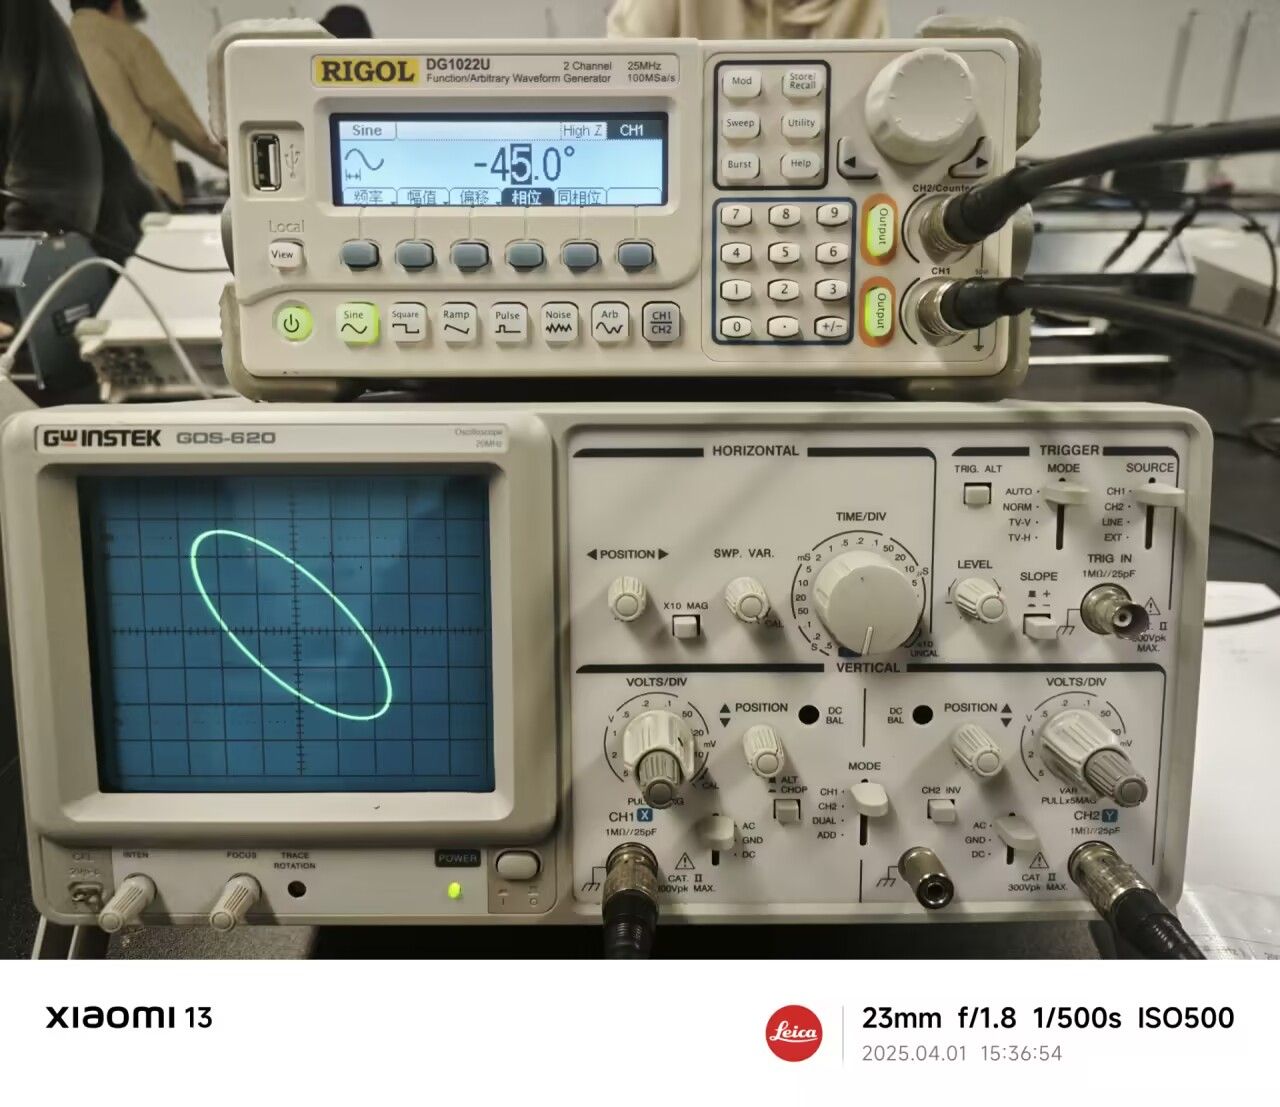
\includegraphics[width=\textwidth]{225.jpg}
			\caption{$\phi_1-\phi_2=5\pi/4$}
			\label{fig:sub5pi4}
		\end{subfigure}
		\hfill
		\begin{subfigure}[b]{0.23\textwidth}
			\centering
			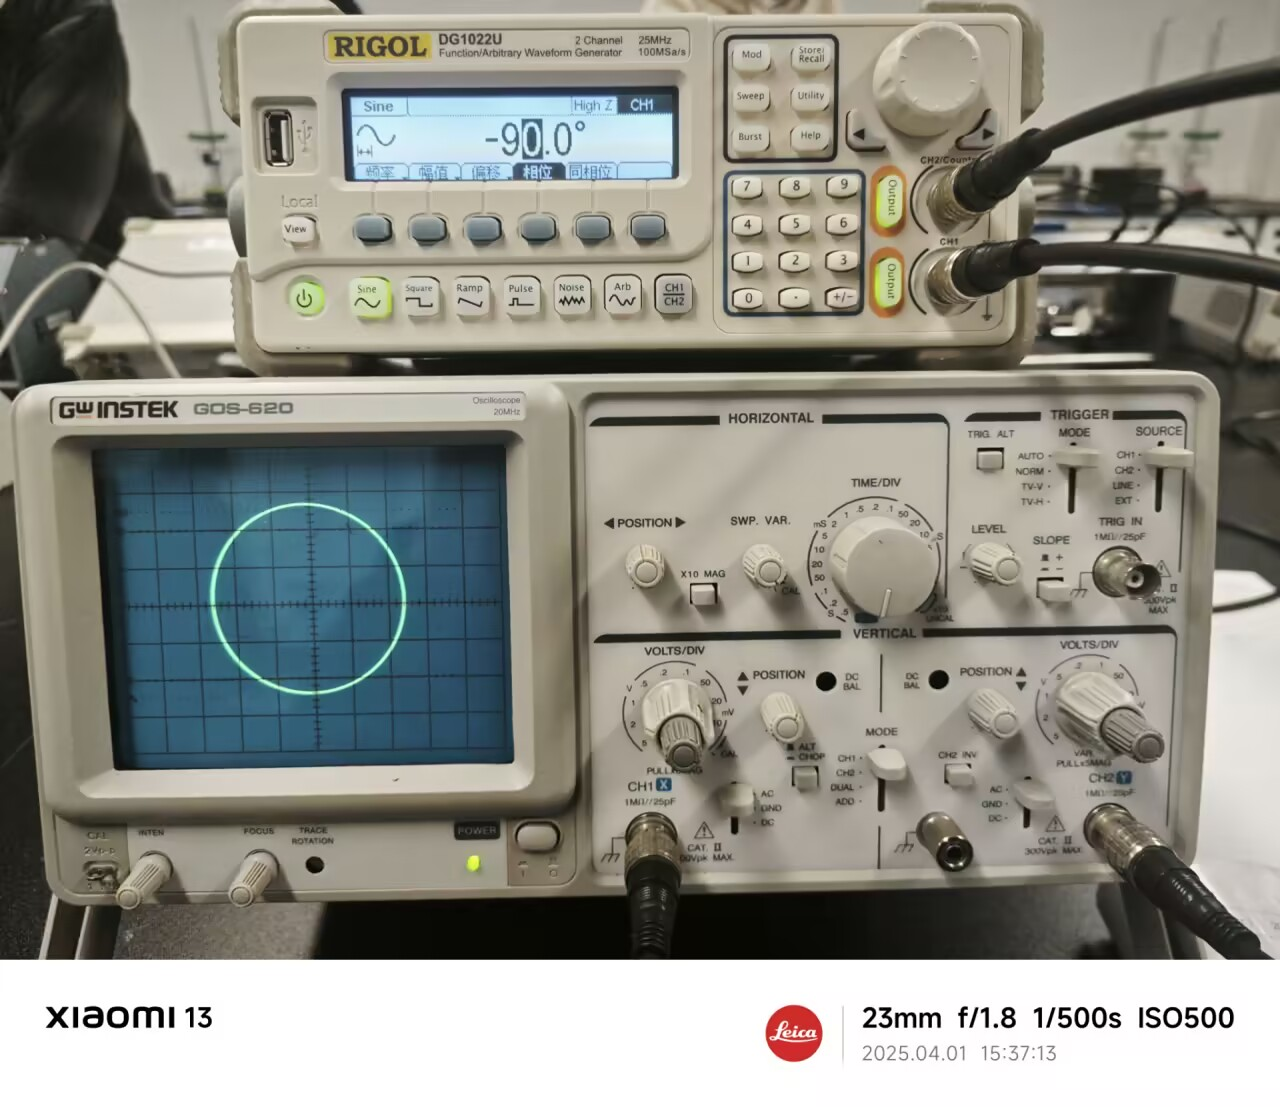
\includegraphics[width=\textwidth]{270.jpg}
			\caption{$\phi_1-\phi_2=3\pi/2$}
			\label{fig:sub3pi2}
		\end{subfigure}
		\hfill
		\begin{subfigure}[b]{0.23\textwidth}
			\centering
			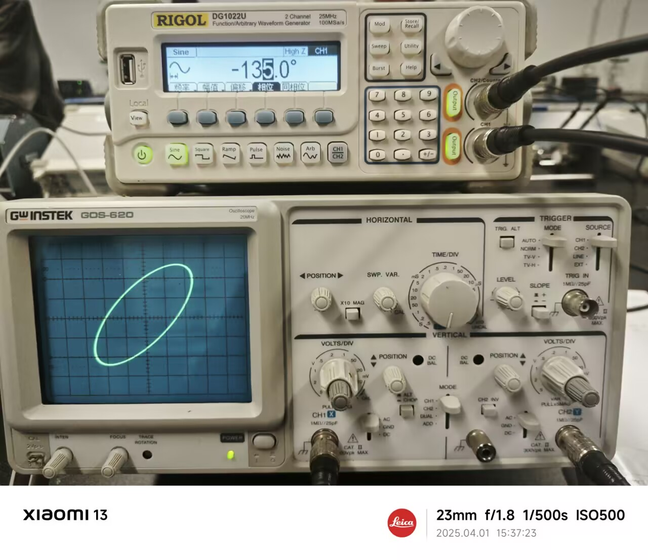
\includegraphics[width=\textwidth]{315.jpg}
			\caption{$\phi_1-\phi_2=7\pi/4$}
			\label{fig:sub7pi4}
		\end{subfigure}
		
		\caption{逐步变化的相位差图(以$\pi/4$间隔)}
		\label{fig:chart2}
	\end{figure}

	不同频率同相位的李萨如图形
	\begin{figure}[H]
		\centering
		% 展示经过化简分数的李萨如图形
		\begin{subfigure}[b]{0.23\textwidth}
			\centering
			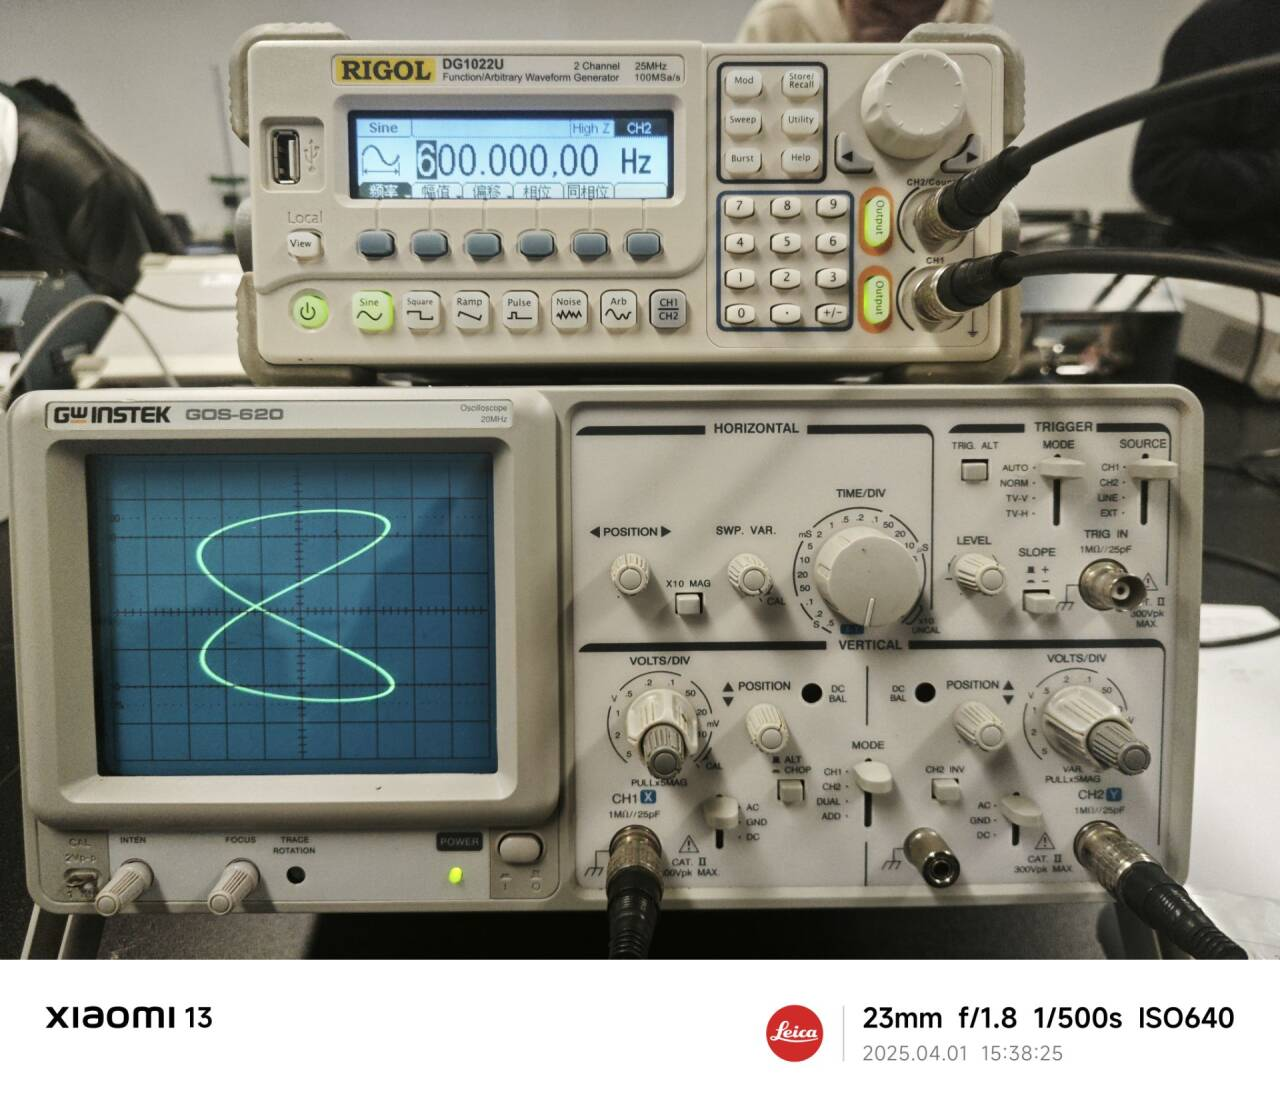
\includegraphics[width=\textwidth]{600.jpg}
			\caption{$f_y/f_x=\dfrac{1}{2}$}
			\label{fig:subLissajous1-2}
		\end{subfigure}
		\hfill
		\begin{subfigure}[b]{0.23\textwidth}
			\centering
			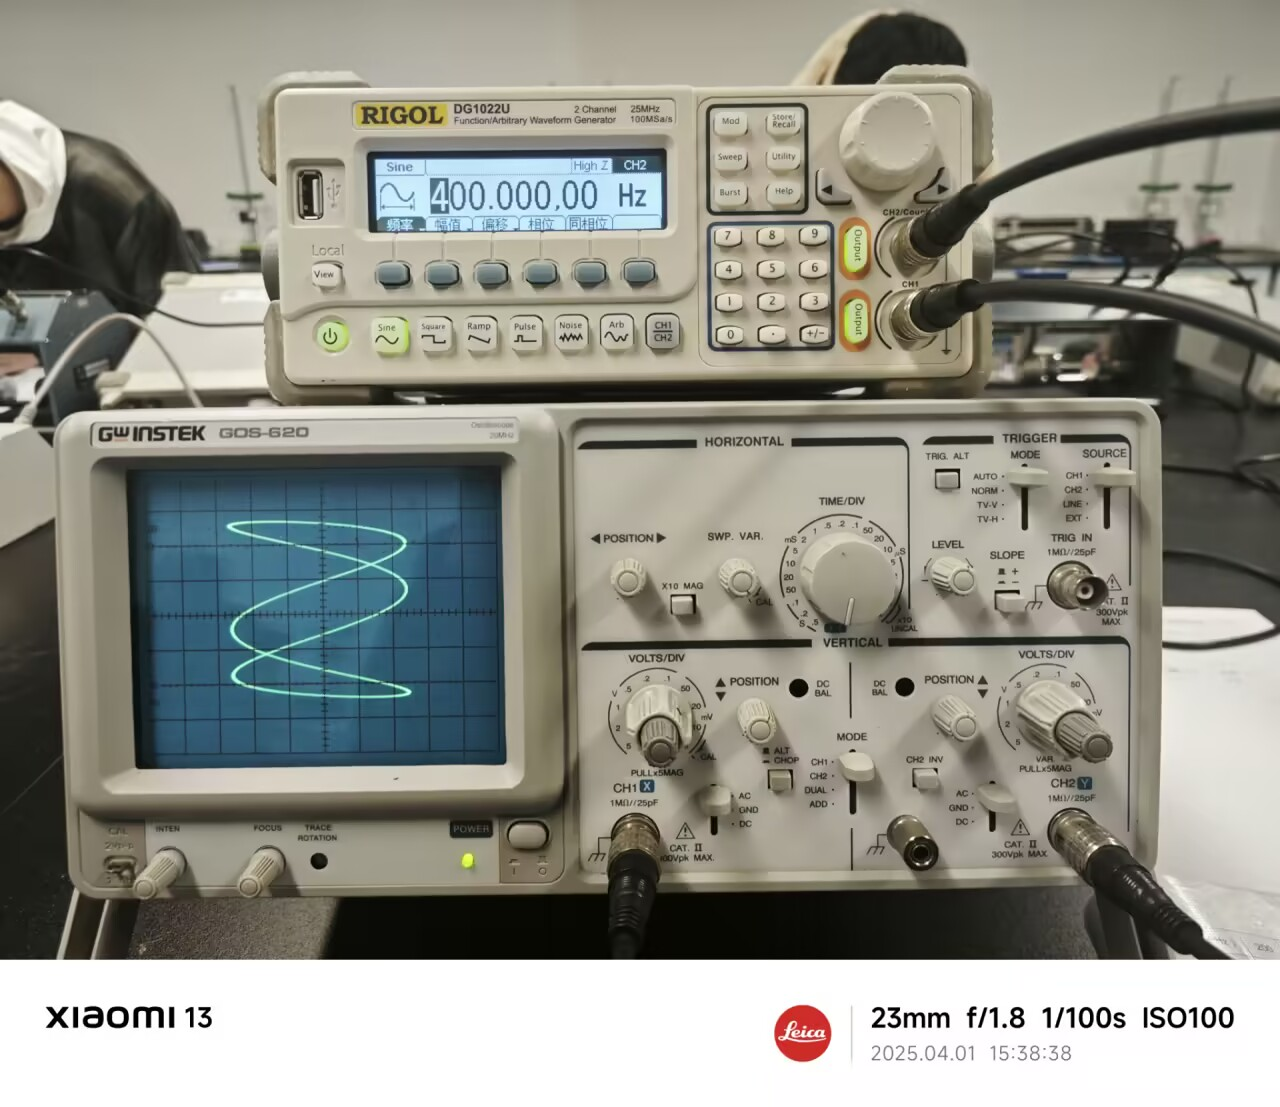
\includegraphics[width=\textwidth]{400.jpg}
			\caption{$f_y/f_x=\dfrac{1}{3}$}
			\label{fig:subLissajous2-2}
		\end{subfigure}
		\hfill
		\begin{subfigure}[b]{0.23\textwidth}
			\centering
			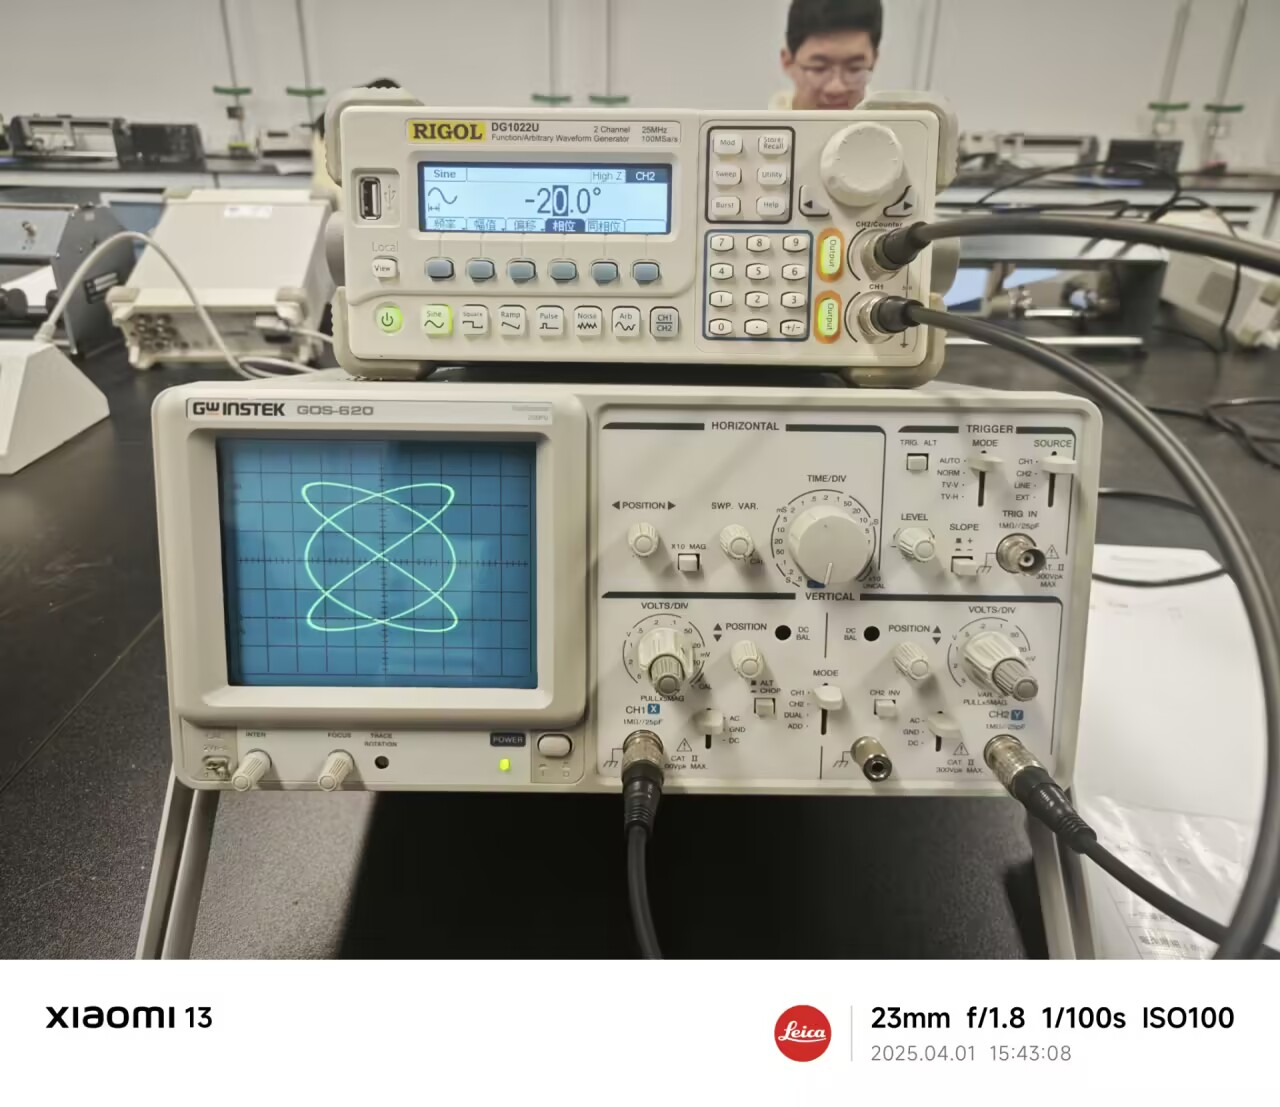
\includegraphics[width=\textwidth]{800.jpg}
			\caption{$f_y/f_x=\dfrac{2}{3}$}
			\label{fig:subLissajous3-2}
		\end{subfigure}
		\hfill
		\begin{subfigure}[b]{0.23\textwidth}
			\centering
			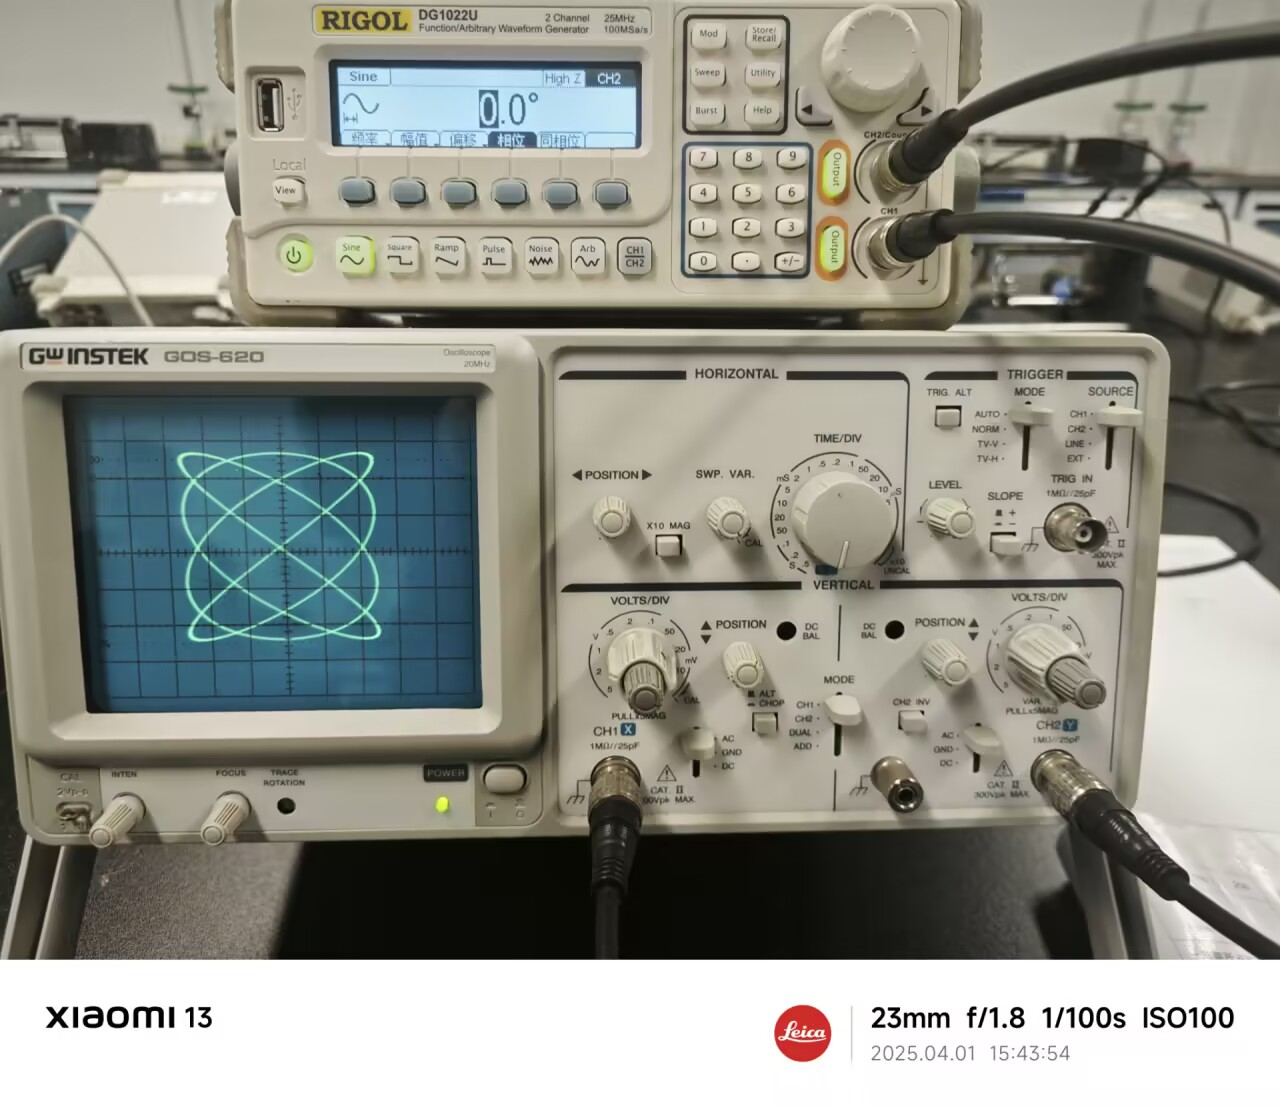
\includegraphics[width=\textwidth]{900.jpg}
			\caption{$f_y/f_x=\dfrac{3}{4}$}
			\label{fig:subLissajous4-2}
		\end{subfigure}
		
		\caption{不同频率同相位的李萨如图形(分数已化简)}
		\label{fig:chart3-simplified}
	\end{figure}

	
	\section{误差分析}
	\begin{enumerate}
		\item 仪器有固有误差,如各信号处理,放大器有精度限制。可换用精度更高的示波器。
		\item 处理信号时可能有噪声,产生随机误差。
		\item 波形有一定宽度,箱光线与腔线间有视差,有读数误差。可调节扫描描参改成大波形,提升读数准确度。
	\end{enumerate}

	\section{思考题}
	\paragraph{1V峰峰值的正弦波,它的有效值是多少?\\}
	对于正弦波,1V峰峰值表示波形正、负峰间的总电压为1V,故其峰值为 
	\[
	V_p = \frac{1\,\mathrm{V}}{2} = 0.5\,\mathrm{V},
	\]
	从而有效值为
	\[
	V_{\mathrm{RMS}} = \frac{V_p}{\sqrt{2}} = \frac{0.5}{\sqrt{2}} \approx 0.3536\,\mathrm{V}.
	\]
	
	(注:若题目中给定1V为峰值,则有效值为 \(1/\sqrt{2}\approx 0.7071\,\mathrm{V}\).)
	
	\paragraph{示波器稳定显示周期信号的条件?\\}
	要使示波器稳定显示周期信号,必须满足以下条件:
	\begin{enumerate}
		\item \textbf{正确的触发设置}:触发电平选在信号幅值范围内,并选择合适的触发沿(上升或下降),确保每次触发采样到相同波形部分;
		\item \textbf{合理的时基设置}:扫描时基应与信号周期匹配,保证屏幕上能完整显示一个或多个周期的波形;
		\item \textbf{信号的稳定性}:输入信号必须为稳定的周期信号,即频率和幅值基本保持恒定。
	\end{enumerate}
	
	
	\section{实验结论}
	本实验利用示波器测量了内置校准信号,信号发生器输出的方波、正弦波的周期、频率及幅度,绘制了校准曲线,验证了李萨如图形。

\end{document}
